% !TEX root=formulas-trigonometria.tex
% Author: Alfredo Sánchez Alberca (asalber@ceu.es)

\sloppy

\section*{Fórmulas de Trigonometría}

\footnotesize
\tcbset{enhanced, colback=color1!10, colframe=color1, fonttitle=\bfseries\large\sffamily, %lifted shadow={1mm}{-2mm}{3mm}{0.1mm}
}

\begin{multicols}{2}

\begin{tcolorbox}[hbox, title=Razones rigonométricas en un triángulo rectángulo]
\begin{minipage}{0.4\textwidth}
\flushleft
\rule{0.4\textwidth}{0pt}
\begin{center}
\begin{tikzpicture}
\coordinate (C) at (-1.5,-1);
\coordinate (A) at (1.5,-1);
\coordinate (B) at (1.5,1);
\draw (C) -- node[above] {$h$} (B) -- node[right] {$o$} (A) -- node[below] {$a$} (C);
\draw (A) +(-.25,0) |- +(0,.25);
\pic [draw, angle radius=1cm, "$\theta$"] {angle=A--C--B};
\end{tikzpicture}
\end{center}
\begin{description}
\item[Seno] $\sen(\theta)=\dfrac{o}{h}$.
\item[Coseno] $\cos(\theta)=\dfrac{a}{h}$.
\item[Tangente] $\tg(\theta)=\dfrac{o}{a}=\dfrac{\sin(\theta)}{\cos(\theta)}$.
\item[Secante] $\sec(\theta)=\dfrac{h}{a}=\dfrac{1}{\cos(\theta)}$.
\item[Cosecante] $\cosec(\theta)=\dfrac{h}{o}=\dfrac{1}{\sen(\theta)}$.
\item[Cotangente] $\ctg(\theta)=\dfrac{a}{o}=\dfrac{\cos(\theta)}{\sen(\theta)}=\dfrac{1}{\tg(\theta)}$.
\end{description}
\end{minipage}
\end{tcolorbox}

\begin{tcolorbox}[hbox, title=Razones trigonométricas en el círculo unitario]
\begin{minipage}{0.4\textwidth}
\resizebox{\textwidth}{!}{
\begin{tikzpicture}
\tikzset{>=stealth}
% draw axises and labels. We store a single coordinate to have the
% direction of the x axis
\draw[->] (-4,0) -- ++(8,0) coordinate (X) node[below] {$x$};
\draw[->] (0,-4) -- ++(0,8) node[left] {$y$};
\draw (3,1pt) -- (3,-1pt) node[anchor = north west] {$1$};
\draw (1pt,3) -- (-1pt,3) node[anchor = south east] {$1$};
\draw (-3,1pt) -- (-3,-1pt) node[anchor = north east] {$-1$};
\draw (1pt,-3) -- (-1pt,-3) node[anchor = north east] {$-1$};

\newcommand\CircleRadius{3cm}
\draw (0,0) circle (\CircleRadius);
% special method of noting the position of a point
\coordinate (P) at (140:\CircleRadius);

\draw[very thick] (0,0) coordinate (O) % store origin
node[below right] {$O$} % label
--
node[above left,pos=1] {$P(x,y)$} % some labels
node[above right,midway] {$r=1$}
(P)
--
node[midway,left] {$y$}
(P |- O) coordinate (Px) % projection onto horitontal line through
% O, saved for later
--
node[midway,below] {$x$}
cycle % closed path
% pic trick is from the angles library, requires the three points of
% the marked angle to be named
pic [draw,->,angle radius=1cm,pic text=$\theta$,
angle eccentricity=1.3] {angle=X--O--P};

% right angle marker
\draw ($(Px)+(0.3,0)$) -- ++(0,0.3) -- ++(-0.3,0);
\end{tikzpicture}
}

\[\cos(\theta)=x \quad \sen(\theta)=y \quad \tg(\theta)=\dfrac{y}{x}\]
\end{minipage}
\end{tcolorbox}

\begin{tcolorbox}[hbox, title=Razones trigonométricas de los principales ángulos]
\begin{minipage}{0.4\textwidth}
\resizebox{\textwidth}{!}{
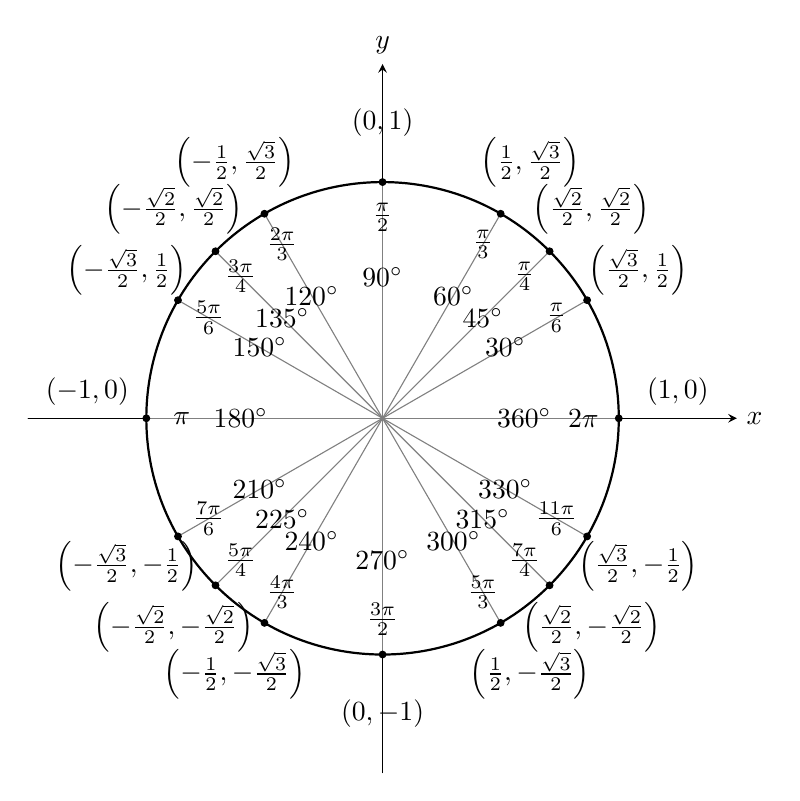
\begin{tikzpicture}[scale=3, cap=round, >=stealth]
% draw the coordinates
\draw[->] (-1.5cm,0cm) -- (1.5cm,0cm) node[right] {$x$};
\draw[->] (0cm,-1.5cm) -- (0cm,1.5cm) node[above] {$y$};

% draw the unit circle
\draw[thick] (0cm,0cm) circle(1cm);

\foreach \x in {30,60,...,360} {
% lines from center to point
\draw[gray] (0cm,0cm) -- (\x:1cm);
% dots at each point
\filldraw[black] (\x:1cm) circle(0.4pt);
% draw each angle in degrees
\draw (\x:0.6cm) node[] {$\x^\circ$};
}
\draw[gray] (0cm,0cm) -- (45:1cm);
\draw[gray] (0cm,0cm) -- (135:1cm);
\draw[gray] (0cm,0cm) -- (225:1cm);
\draw[gray] (0cm,0cm) -- (315:1cm);
\filldraw[black] (45:1cm) circle(0.4pt);
\filldraw[black] (135:1cm) circle(0.4pt);
\filldraw[black] (225:1cm) circle(0.4pt);
\filldraw[black] (315:1cm) circle(0.4pt);
\draw (45:0.6cm) node[] {$45^\circ$};
\draw (135:0.6cm) node[] {$135^\circ$};
\draw (225:0.6cm) node[] {$225^\circ$};
\draw (315:0.6cm) node[] {$315^\circ$};

% draw each angle in radians
\foreach \x/\xtext in {
30/\frac{\pi}{6},
45/\frac{\pi}{4},
60/\frac{\pi}{3},
90/\frac{\pi}{2},
120/\frac{2\pi}{3},
135/\frac{3\pi}{4},
150/\frac{5\pi}{6},
180/\pi,
210/\frac{7\pi}{6},
225/\frac{5\pi}{4},
240/\frac{4\pi}{3},
270/\frac{3\pi}{2},
300/\frac{5\pi}{3},
315/\frac{7\pi}{4},
330/\frac{11\pi}{6},
360/2\pi}
\draw (\x:0.85cm) node[] {$\xtext$};

\foreach \x/\xtext/\y in {
% the coordinates for the first quadrant
30/\frac{\sqrt{3}}{2}/\frac{1}{2},
45/\frac{\sqrt{2}}{2}/\frac{\sqrt{2}}{2},
60/\frac{1}{2}/\frac{\sqrt{3}}{2},
% the coordinates for the second quadrant
150/-\frac{\sqrt{3}}{2}/\frac{1}{2},
135/-\frac{\sqrt{2}}{2}/\frac{\sqrt{2}}{2},
120/-\frac{1}{2}/\frac{\sqrt{3}}{2},
% the coordinates for the third quadrant
210/-\frac{\sqrt{3}}{2}/-\frac{1}{2},
225/-\frac{\sqrt{2}}{2}/-\frac{\sqrt{2}}{2},
240/-\frac{1}{2}/-\frac{\sqrt{3}}{2},
% the coordinates for the fourth quadrant
330/\frac{\sqrt{3}}{2}/-\frac{1}{2},
315/\frac{\sqrt{2}}{2}/-\frac{\sqrt{2}}{2},
300/\frac{1}{2}/-\frac{\sqrt{3}}{2}}
\draw (\x:1.25cm) node[] {$\left(\xtext,\y\right)$};

% draw the horizontal and vertical coordinates
% the placement is better this way
\draw (-1.25cm,0cm) node[above=1pt] {$(-1,0)$}
(1.25cm,0cm)  node[above=1pt] {$(1,0)$}
(0cm,-1.25cm) node[] {$(0,-1)$}
(0cm,1.25cm)  node[] {$(0,1)$};
\end{tikzpicture}
}
\end{minipage}
\end{tcolorbox}

\begin{tcolorbox}[hbox, title=Conversión de ángulos]
\begin{minipage}{0.4\textwidth}
\begin{description}
\item[Grados a radianes] $y=\dfrac{\pi \mbox{rad}}{180^\circ}x$.
\item[Radianes a grados] $y=\dfrac{180^\circ}{\pi \mbox{rad}}x$.
\end{description}
\end{minipage}
\end{tcolorbox}

\begin{tcolorbox}[hbox, title=Teorema de pitágoras]
\begin{minipage}{0.4\textwidth}
\begin{center}
\begin{tikzpicture}
\coordinate (C) at (-1.5,-1);
\coordinate (A) at (1.5,-1);
\coordinate (B) at (1.5,1);
\draw (C) -- node[above] {$h$} (B) -- node[right] {$o$} (A) -- node[below] {$a$} (C);
\draw (A) +(-.25,0) |- +(0,.25);
\pic [draw, angle radius=1cm, "$\theta$"] {angle=A--C--B};
\end{tikzpicture}
\end{center}
\[
\renewcommand{\arraystretch}{1.5}
\begin{array}{c}
a^2 + o^2 = h^2                     \\
\sen(\theta)^2 + \cos(\theta)^2 = 1 \\
1+\tg(\theta)^2 = \sec(\theta)^2    \\
1+\ctg(\theta)^2 = \cosec(\theta)^2
\end{array}
\]
\end{minipage}
\end{tcolorbox}

\begin{tcolorbox}[hbox, title=Razones trigonométicas de sumas de ángulos]
\begin{minipage}{0.4\textwidth}
\[
\renewcommand{\arraystretch}{1.5}
\begin{array}{c}
\sen(\alpha+\beta)=\sen(\alpha)\cos(\beta)+\cos(\alpha)\sen(\beta) \\
\sen(\alpha-\beta)=\sen(\alpha)\cos(\beta)-\cos(\alpha)\sen(\beta) \\
\cos(\alpha+\beta)=\cos(\alpha)\cos(\beta)-\sen(\alpha)\sen(\beta) \\
\cos(\alpha-\beta)=\cos(\alpha)\cos(\beta)+\sen(\alpha)\sen(\beta) \\
\sen(2\theta)=2\sen(\theta)\cos(\theta)                            \\
\cos(2\theta)=\cos(\theta)^2-\sen(\theta)^2
\end{array}
\]
\end{minipage}
\end{tcolorbox}

\begin{tcolorbox}[hbox, title=Teoremas de los senos y los cosenos]
\begin{minipage}{0.4\textwidth}
\begin{center}
\begin{tikzpicture}
\newcommand\XB{4}
\newcommand\ALPHA{30}
\newcommand\XC{{(\XB*(cos(\ALPHA)*cos(\ALPHA) - sin(\ALPHA)*sin(\ALPHA)) + \XB)*0.5}}
\newcommand\YC{{sqrt(cos(\ALPHA)*\XB*cos(\ALPHA)*\XB - (\XB*(cos(\ALPHA)*cos(\ALPHA) - sin(\ALPHA)*sin(\ALPHA)) + \XB)*0.5*(\XB*(cos(\ALPHA)*cos(\ALPHA) - sin(\ALPHA)*sin(\ALPHA)) + \XB)*0.5)}}
% Draw the triangle
\draw (0,0) coordinate (A) -- (\XC,\YC) coordinate (C) -- (\XB,0) coordinate (B) -- (0,0);
% Draw edge text
\node (c) at ($(A)!0.5!(B)$) [below] {c};
\node (b) at ($(A)!0.5!(C)$) [above] {b};
\node (a) at ($(B)!0.6!(C)$) [right] {a};
% draw angles
\draw (0,0) -- (0:0.75cm) arc (0:\ALPHA:.75cm);
\coordinate[label=right:$\alpha$] (Alpha) at (0.25,0.15);
\begin{scope}[shift={(\XB,0)}]
\draw(0,0) -- (-180:0.50cm) arc (180:{180-(90-\ALPHA)}:0.5cm);
\draw (150:0.35cm) node {$\beta$};
\end{scope}
\begin{scope}[shift={(\XC, \YC)}]
\draw (0,0) -- ({180+\ALPHA}:0.5cm) arc ({180+\ALPHA}:{180+\ALPHA+90}:0.5cm);
\draw (-0.1,-0.05) node[below] {$\gamma$};
\end{scope}
\end{tikzpicture}
\end{center}
\begin{description}
\item[Teorema de los senos]
      \[\frac{a}{\sen(\alpha)}=\frac{b}{\sen(\beta)}=\frac{c}{\sen(\gamma)}\]
\item[Teorema de los cosenos]
      \[
      \renewcommand{\arraystretch}{1.5}
      \begin{array}{c}
      a^2 = b^2 + c^2 - 2bc\cos(\alpha) \\
      b^2 = a^2 + c^2 - 2ac\cos(\beta)  \\
      c^2 = a^2 + b^2 - 2ab\cos(\gamma)
      \end{array}
      \]
\end{description}
\end{minipage}
\end{tcolorbox}


\end{multicols}

